\documentclass{article}
\usepackage[utf8]{inputenc}
\usepackage[brazilian]{babel}
\setlength{\voffset}{0pt}
\usepackage[bottom=2cm,top=2cm,left=3cm,right=2cm]{geometry}
\usepackage{amsmath,amssymb,amsthm}
\usepackage{gensymb}
\usepackage{graphicx}
\usepackage{grffile}
\usepackage[section]{placeins}
\title{EP1 - Relatório}
\author{Lucas Seiki Oshiro - 9298228\\ Marcos Vinicius do Carmo Sousa    - 9298274}

\begin {document}
\maketitle
\section{ Parte 1: Aritmética de Ponto Flutuante}
\paragraph*{1.}
\subparagraph{a)}
O maior número que pode ser representado é aquele com todos os bits b2 ... b24 = 1 e o maior expoente E possível (ou seja, 126). Ou seja, é o número $(1 * 2^{-1} + \sum_{i = 2}^{24} (1 * 2^{-i})) * 2^{126} = (1 - 2^{24}) * 2^{126}$.

\subparagraph{b)}
O menor número positivo é o que tem os bits b2, b3 ...,b24 = 0, e o menor expoente E possível (ou seja, -127). Dessa forma, esse número é $(1 * 2^{-1} + \sum_{i = 2}^{24} (0 * 2^{-i})) * 2^{-127} = 2^{-1} * 2^{-127} = 2^{-128}$.

\subparagraph{c)}
O menor inteiro positivo não represetável nesse sistema é o numero caso a mantissa tivesse a precisao do expoente E com b2 ... b24 = 1 e b25 ... b125 = 0 e b126 = 1 e com o expoente E = 126.


\paragraph*{2.}
\subparagraph{I - $1/10$}

 O número 1/10 é escrito na base binária como a dízima periódica $(0.0001100110011...)_{2}$, ou seja, $(1.1001100110011001100110011...) * 2^{-4}$.
 
 Como o número é positivo, o bit de sinal vale 0.
 
 Como o expoente é -4, o bitstring do expoente é a representação binária de $-4 + 127 = 123$ com 8 dígitos, ou seja, 01111011.
 
 Arredondamento para baixo: a mantissa será 1.10011001100110011001100, logo o número é armazenado como 00111101110011001100110011001100.
 
 Arredondamento para cima: a mantissa será 1.10011001100110011001101, logo o número é armazenado como 00111101110011001100110011001101.
 
 Arredondamento em direção ao zero: a mantissa será 1.10011001100110011001100, logo o número é armazenado como 00111101110011001100110011001100.
 
 Arredondamento para o mais próximo: a mantissa será 1.10011001100110011001100, logo o número é armazenado como 00111101110011001100110011001100.
 
 \subparagraph{II - $1 + 2^{-25}$}
 O número $1 + 2^{-25}$ é escrito na base binária como $(1.0000000000000000000000001)_{2}$, ou seja, $(1.0000000000000000000000001)_{2} * 2^{0}$.
 
 Como o número é positivo, o bit de sinal vale 0.
 
 Como o expoente é 0, o bitstring do expoente é a representação binária de 0 + 127 = 127 com 8 dígitos, ou seja, 01111111.
 
 Arredondamento para baixo: a mantissa será 1.00000000000000000000000, logo o número é armazenado como 00111111100000000000000000000000.
 
 Arredondamento para cima: a mantissa será 1.00000000000000000000001, logo o número é armazenado como 00111111100000000000000000000001.
 
 Arredondamento em direção ao zero: a mantissa será 1.00000000000000000000000, logo o número é armazenado como 00111111100000000000000000000000.
 
 Arredondamento para o mais próximo a mantissa será 1.00000000000000000000000, logo o número é armazenado como 00111111100000000000000000000000.
 
\subparagraph{III - $2^{130}$}
O número $2^{130}$ é maior do que o maior número que pode ser representado no formato IEEE single.

Arredondamento para baixo: será subsituído pelo maior número normalizado do formato IEEE single, ou seja, será representado como 01111111011111111111111111111111.

Arredondamento para cima: será subistituído por $+\infty$, ou seja, será representado como 01111111100000000000000000000000.

Arredondamento em direção ao zero: como $2^{130}$ é positivo, o número é arredondado para baixo, ou seja, será representado como 01111111011111111111111111111111.

Arredondamento para o mais próximo: como o número Nmax (maior número normalizado do formato IEEE single) é $2^{128}$, sua ulp vale $2^{127}$. Como $2^{128} > 2^{128} + 2^{127}$, o número é arredondado para $+\infty$, ou seja, será representado como 01111111011111111111111111111111.

\paragraph*{3.}
O maior número de ponto flutuante x tal que 1 + x é igual a 1, arredondando para o mais próximo no formato IEEE single, é $2^{-24}$.
Isso ocorre porque o número 1 + $2^{-24}$ é a média aritmética entre 1 e 1 + $2^{-23}$, ou seja, ambos os números são os mais próximos, e nesses casos o número é arredondado para aquele que contém o número 1 em seu bit menos significativo.

Já no caso do formato IEEE double, o maior número de ponto flutuante x tal que 1 + x é igual a 1, arredondando para o mais próximo é $2^{-53}$.
Uma vez que 1 + $2^{-53}$ é a média entre 1 e 1 + $2^{-52}$, sendo assim, da mesma forma, é arredondado para 1 por ambos os números 1 e 1 + $2^{-52}$ serem os mais próximos e 1 ser a opção com o último bit igual a 1.

\paragraph*{4.}
\subparagraph{Comutatividade:}
A soma em ponto flutuante ser comutativa significa que a igualdade $x \ \oplus y = y \oplus x$\footnote{Considerando como $\oplus$ a soma de ponto flutuante} é verdadeira e ela equivale à igualdade\footnote{Considerando round($x$) o valor arredondado de x num sistema de ponto flutuante} round(round($x$) + round($y$) = round(round($y$) + round($x$)), sendo $x$ e $y$ números que podem ser representados num sistema de ponto flutuante. 

Pela propriedade comutativa da soma aritmética, temos então que round($x$) + round($y$) = round($y$) + round($x$).

Como o arredondamento para um mesmo número é sempre igual, o valor de round(round($x$) + round($y$) sempre será igual ao de round(round($y$) + round($x$)). Sendo assim, a soma em ponto flutuante é comutativa. $\square$

\subparagraph{Associatividade:}
Para que soma em ponto flutuante seja associativa é necessária ser verdadeia a hipótese que $x \oplus (y \oplus z) = (x \oplus y) \oplus z$, em outras palavras, round(round($x$) + round(round($y$) + round($z$))) = round(round(round($x$) + round($y$)) + round($z$))).

Pode-se reescrever essa igualdade como round($x$) + round(round($y$) + round($z$)) + $e_{1}$ = round(round($x$) + round($y$)) + round($z$)) + $e_{2}$, sendo $e_{1}$ e $e_{2}$ os erros dos arredondamentos das expressões.

Pode-se, ainda, reescrever a mesma igualdade como round($x$) + round($y$) + round($z$) + $e_{y+z}$ + $e_{1}$ = round($x$) + round($y$) + round($z$) + $e_ {x+y}$ + $e_{2}$, com $e_{y+z}$ sendo o erro do arredondamento de round($y$) + round($z$) e $e_ {x+y}$ o erro do arredondamento de round ($x$) + round($y$).

Dessa forma, temos que $e_{y+z}$ + $e_{1}$ = $e_ {x+y}$ + $e_{2}$. Essa afirmação não é verdadeira, uma vez que iguala somas de erros que ocorreram em processos independentes, ou seja, nada se pode concluir dessas somas. Isso contradiz a hipótese inicial, portanto, a associatividade não é aplicável à soma em ponto flutuante. $\square$

\section{Parte II - Método de Newton}
\subsection{Implementação}
A função newton () calcula uma raiz de uma função, usando o método de Newton, a partir de um dado $x_{0}$. Caso a derivada da função em $x_{0}$ seja igual a zero, ou caso o método de newton seja iterado mais que 100 vezes, a função devolve NaN. O valor é arredondado para ter no máximo 15 casas decimais, a fim de que possa ser comparado com o valor de outras raízes.

Para cada ponto do quadrado de largura $n$ pixels, é associado um valor entre $-2$ e $2$, e entre $-2i$ e $2i$, sendo esses valores usados como $x_{0}$ para calcular o método de Newton.

A função newton{\_}basins () itera sobre o valores de cada pixel, e calcula a convergência do método de Newton a partir de cada um, sendo que os valores (e NaN, indicando que não há convergência) achados são adicionados num vetor, e os índices do vetor são a representação da raiz, que será impressa no arquivo de saída.

Para utilizar a função newton{\_}basins (), deve-se abrir o octave no mesmo diretório do arquivo newton{\_}basins e usar como argumentos o vetor de coeficientes da função polinomial a ser analisada, e o valor n, tal que o quadrado gerado tenha lado $n^{2}$.

\subsection{Experimentos}
As figuras a seguir são o resultado dos experimentos com cada umas das funções indicadas na legenda.
\begin{figure}[!hbt]
	\centering
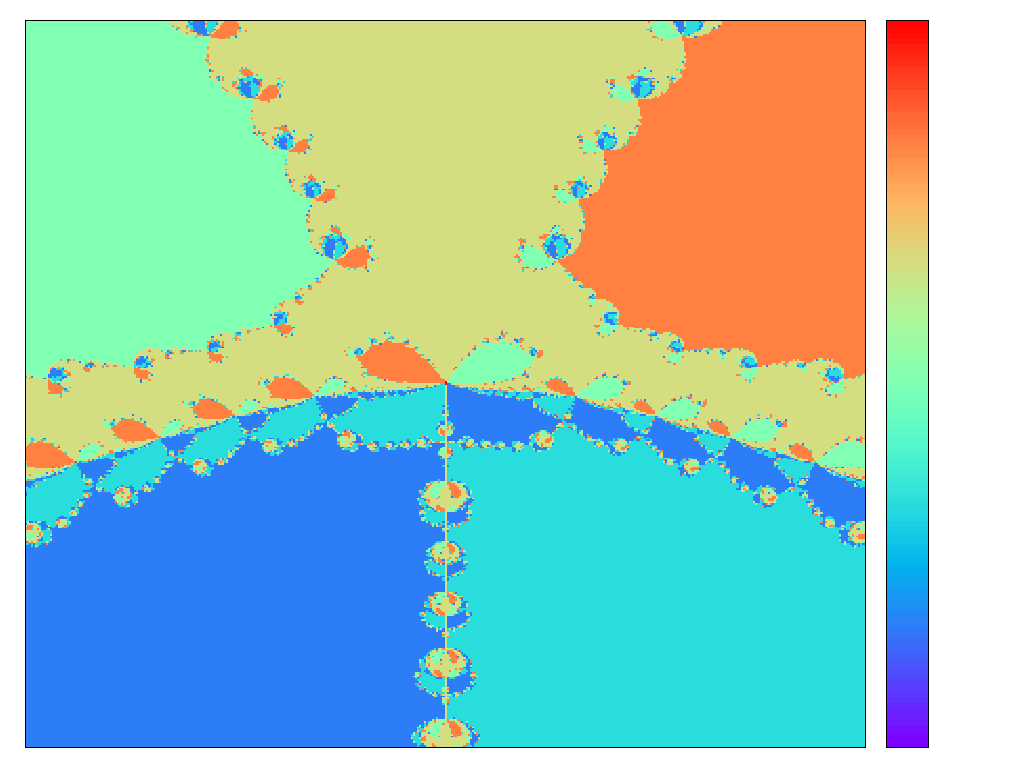
\includegraphics[width=0.7\linewidth]{imagens/1_-1_0_1_0_-1.png}
\caption{$f(x) = x^{5} - x^{4} + x^{2} - 1$}
\end{figure}

\begin{figure}[!hbt]
	\centering
	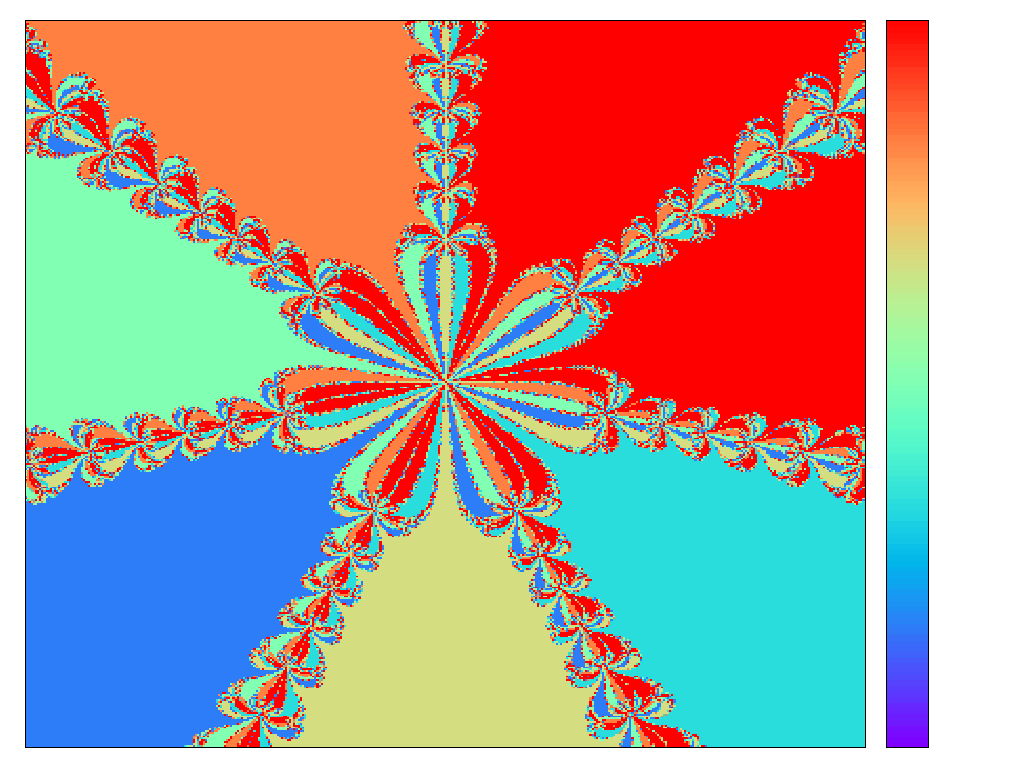
\includegraphics[width=0.7\linewidth]{imagens/[1, 0, 0, 0, 0, 0, 0, 1].png}
	\caption{$f(x) = x^{7} + 1$}
\end{figure}

\begin{figure}[!hbt]
	\centering
	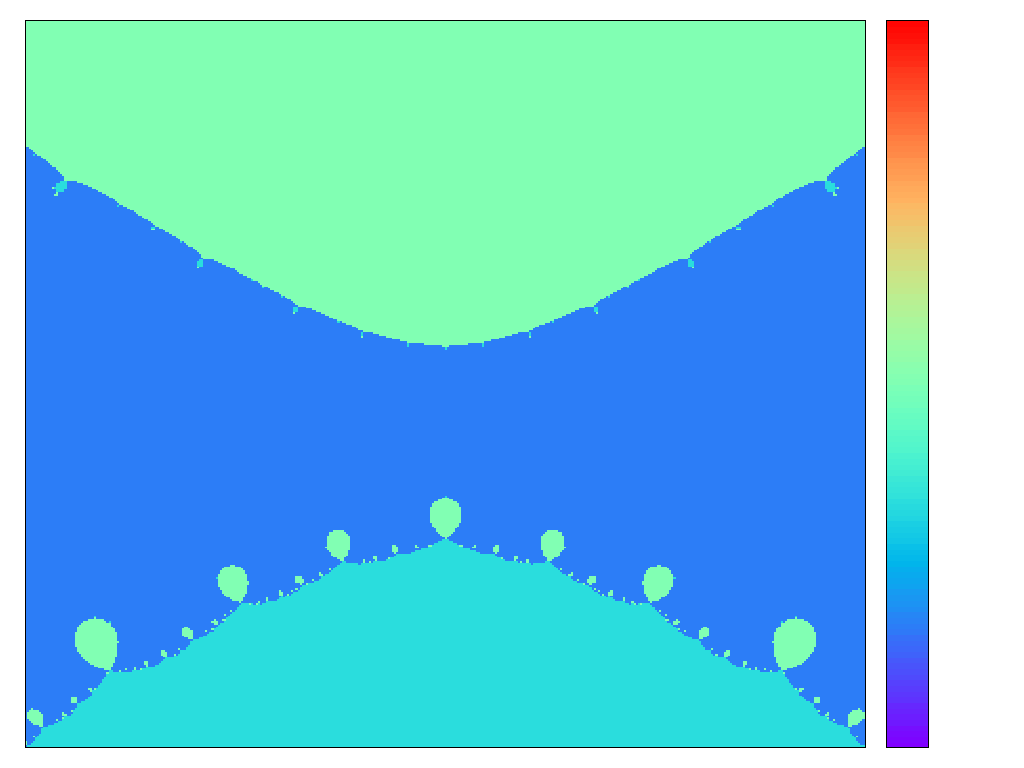
\includegraphics[width=0.7\linewidth]{imagens/[2, 2, -1, 0].png}
	\caption{$f(x) = 2x^{3} + 2x^{2} - x$}
\end{figure}

\begin{figure}[!hbt]
	\centering
	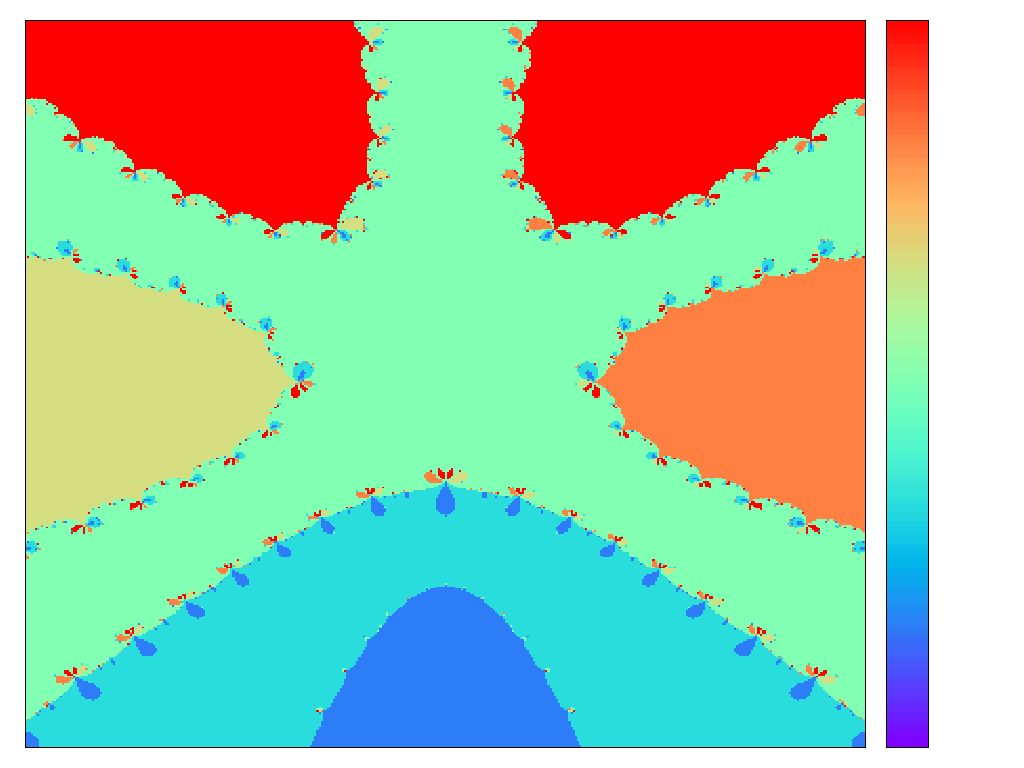
\includegraphics[width=0.7\linewidth]{imagens/[1, 0, -1, 1, 0, 1, 2, 0].png}
	\caption{$f(x) = x^{7} -x^{5} + x^{4} + x^{3} + x^{2} + 2x$}
\end{figure}

\section{Parte III - Encontrando todas as raízes das funções}
\subsection{Implementação}
A função achaRaizes () recebe como parâmetro uma função, sua derivada, o limite inferior do intervalo, o limite superior do intervalo, o número de subintervalos e a tolerância, e imprime as raízes da função dentro das condições dadas. Para usá-la, deve-se chamá-la usando o octave aberto no mesmo diretório do arquivo achaRaizes.m.

Foram criadas duas funções auxiliares no arquivo achaRaizes.m: a função bissec, que calcula uma aproximação de uma raiz de f, usando o método da bissecção com apenas 3 iterações e a função newton (), que calcula raízes usando o método de Newton.

A função newton (), quando calcula a derivada de $f$ num ponto $x_{0}$ e o resultado é zero, incrementa o valor de $x_{0}$ em $0.1$, para que não ocorra divisão por zero, e assim aplica o método de newton a partir de outro ponto.

\subsection{Experimentos}
\begin{itemize}
\item 
	$f(x) \left\{
	\begin{array}{ll}
	sen(x) / x, x \neq 0\\
	1, x = 0
	\end{array}\right.$\\
	
	Foram encontradas as seguintes raízes, no intervalo $[0, 60]$, com 100 subintervalos e tolerância $1.e-8$:
	 3.1416
	 6.2832
	 9.4248
	 12.566
	 15.708
	 18.850
	 21.991
	 25.133
	 28.274
	 31.416
	 34.558
	 37.699
	 40.841
	 43.982
	 47.124
	 50.265
	 53.407
	 56.549
	 59.690
	 
\item
	$f(x) = 2 * cosh (x/4) - x$
	
	Foram encontradas as seguintes raízes, no intervalo $[0, 60]$, com 100 subintervalos e tolerância $10^{-8}$:
	2.3576                                                                                                     	8.5072 
	
\item	
	$f(x) = x^{3} / 3 + x^{2} + sen(x) - e ^{x}$
	
	Foram encontradas as seguintes raízes, no intervalo $[10, 10]$, com 100 subintervalos e tolerância $10^{-8}$:
-2.8911                                                                                                           -1.6078                                                                                                           
1.6369
2.4163

\item	
$f(x) = x ^{5} + x ^{2} - 0.2$

Foram encontradas as seguintes raízes, no intervalo $[10, 10]$, com 100 subintervalos e tolerância $10^{-8}$:
-0.91250
-0.47292
0.43039

\end{itemize}

\end{document}
